\problemname{The Geneva Confection}

In order to ensure peace and prosperity for future generations, the United Nations is creating the
world's largest candy. The ingredients must be taken in railway cars from the top of a mountain and
poured into Lake Geneva. The railway system goes steeply from the mountaintop down to the lake, with
a T-shaped branch in the middle as shown below.

\begin{center}
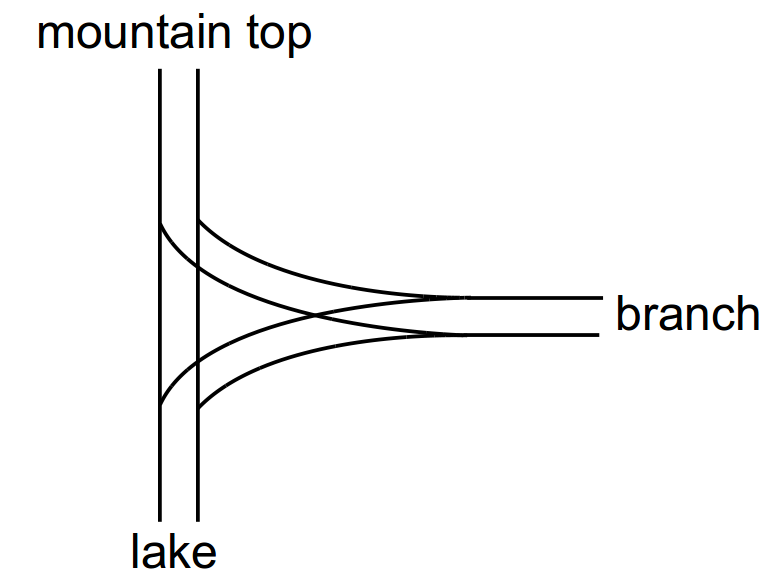
\includegraphics[width=0.4\textwidth]{confection}
\end{center}

Right now, each of the $N$ ingredients is in its own railway car. Each railway car is assigned a
positive integer from $1$ to $N$. The ingredients must be poured into the lake in the order $1, 2,
3, ..., N$ but the railway cars are lined up in some random order. The difficulty is that, because
of the especially heavy gravity today, you can only move cars downhill to the lake, or sideways on
the branch line. Is it still possible to pour the ingredients into the lake in the order $1, 2, 3,
..., N$?

For example, if the cars were in the order $2, 3, 1, 4$, we can slide these into the lake in order as described below:

\begin{minipage}{0.45\linewidth}
  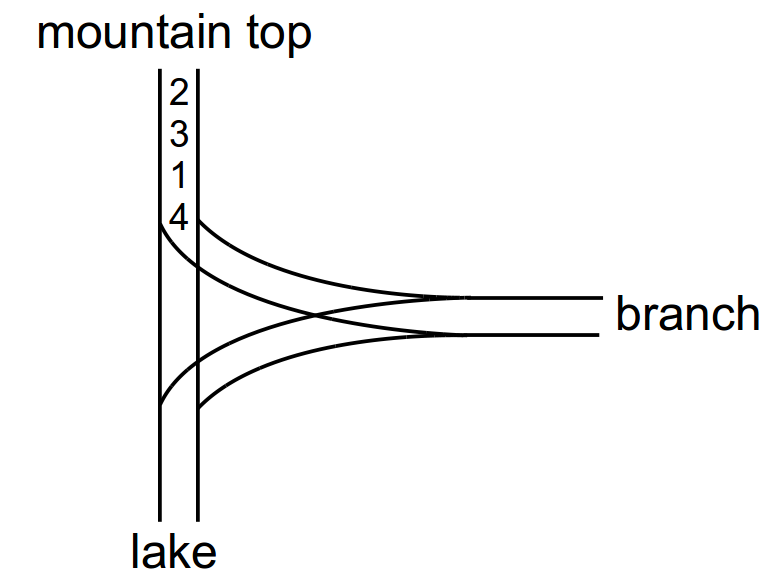
\includegraphics[width=\linewidth]{confection2}
\end{minipage}
\hspace{0.05\linewidth}
\begin{minipage}{0.45\linewidth}
 \begin{itemize}
    \item Slide car 4 out to the branch
    \item Slide car 1 into the lake
    \item Slide car 3 out to the branch
    \item Slide car 2 into the lake
    \item Slide car 3 from the branch into the lake
    \item Slide car 4 from the branch into the lake
  \end{itemize}
\end{minipage}

\section*{Input}
The first line will contain the number $T (1 \leq T \leq 10)$ which is the number of different tests
that will be run. Each test has the form of an integer $N (1 \leq N \leq 100\,000)$ on the first
line of the test, followed by a list of the $N$ cars listed from top to bottom. The cars will always
use the numbers from $1$ to $N$ in some order.

\section*{Output}
For each test, output one line which will contain either ``\verb+Y+'' (for ``yum'') if the recipe can be
completed, and ``\verb+N+'' otherwise.
